\chapter{Preliminaries}
\label{ch:preliminaries}
This chapter provides an overview of the models used for decision tree induction and variable selection. We begin by discussing the earliest methods of induction, greedy algorithms. With the advance of time (about a decade), greedy induction approaches became fully implemented through high quality Fortran code. Bayesian approaches to building decision trees were not possible until advances in computing power and the rediscovery of sampling based approaches to Bayesian statistics became popular again. While the work of Breiman et al. \cite{breiman1984classification} always contained a Bayesian flavor, no probability measure over trees was ever proposed. That is until the groundbreaking works of Denison, Mallick and Smith \cite{denison1998bayesian} and Chipman, George, and Mcculloch \cite{chipman1998bayesian}.

 During the same time (the 1990s and the 2000s), researchers in Machine Learning and Statistics were developing theory beyond that published by Breiman et al. \cite{breiman1984classification}, that ensured decision trees' consistency. In this case consistency means that the error rate of the tree converges to the Bayes error. The initial impetus for this work stemmed from the landmark paper of Vapnik and Chervonenkis \cite{vapnik1971uniform}, and subsequent work by Vapnik \cite{vapnik2000nature}, though it would take over a decade for the full power of their combinatorial approach to be widely used in both Machine Learning and Statistics. 

This chapter presents necessary preliminaries for the reader to understand the developments in subsequent chapters. Therefore the reader may omit this chapter on a first reading and refer back to the necessary subsections when subsequent chapters recall the preliminaries. Section \ref{ch:p1sub_greedy_ind} and Section \ref{ch:p2sub_bayes} review the necessary material on greedy and Bayesian approaches to decision tree induction. Section \ref{ch:p4sub_var_sel} details a similar variable selection approach proposed for decision trees with time series data. This approach, while similar in spirit to our methods, is significantly different in both methodology and application to our methods but we include a discussion of the method for completeness. Finally, Section \ref{ch:p3sub_theory} details how alternative models of a response variable can work and what requirements these alternate models must satisfy. The reader who is not familiar with these two approaches to decision trees should read these two subsections before moving on to the rest of the thesis.  

\section{Greedy Induction}
\label{ch:p1sub_greedy_ind}

In this section we answer the question: how does greedy induction work? Once the reader has completed this section they should, with sufficient time, be able to reproduce computer code that implements decision trees using greedy strategies. We begin with impurity functions. 

\subsection{Impurity Functions}

An impurity function corresponds to a likelihood function in statistics or to an objective function in machine learning. This function measures, in some sense, how many good observations lie in a node of the tree and how many bad observations lie in a node of the tree. Formally, an impurity function, denoted $\phi$, must satisfy three axioms:

\begin{enumerate}
\item $\phi(1/2,1/2) \geq \phi(p, 1-p)$ for any $p\in[0,1]$. 
\item $\phi(0,1)=\phi(1,0)=0$. 
\item $ \phi(p, 1-p)$ non-decreasing for $p\in[0,1/2]$ and non-increasing for $p\in[1/2,1]$. 
\end{enumerate}

Breiman et al. \cite{breiman1984classification} suggest the following impurity functions: 
\begin{enumerate}
\item Entropy: $\phi(p,1-p)= -plog(p) -(1-p)log(1-p)$.
\item Gini: $\phi(p, 1-p)=2p(1-p)$.
\item Misclass probability: $\phi(p, 1-p)=min(p,1-p).$
\end{enumerate}

A visual comparison of these impurity functions  is displayed in Figure \ref{fig:impurity}. 

\begin{figure}[H]
  \centering
  \includegraphics[scale=.7]{figures/impurity_plot.pdf}
  \caption{A plot of the three impurity functions: entropy (solid line), Gini (thatched line), and misclass probability (dots).  }
  \label{fig:impurity}
\end{figure}

To build a regression tree, in place of an impurity function, we use the mean squared error criteria denoted

$$\text{MSE}: \phi(y_i, \bar{y})=\frac{\sum_{i=1}^n(y_i-\bar{y})^2}{n}.$$
The reader should note that the greedy approach to decision tree induction always tries to optimize impurity functions. The optimization problems are known to be NP-Hard (for an introduction to complexity theory confer Garey and Johnson \cite{garey1979computers}). Briefly, NP-Hard optimization problems are considered some of the hardest optimization problems to solve. These optimization problems increase exponentially with the number of observations in the problem. Therefore, exact methods will nearly always take too long to compute and thus greedy strategies are used to approximate the global optimum, assuming one exists, with a local optimum. 
\subsection{Induction}
The induction of decision trees proceeds by solving the objective function

\begin{equation}
\underset{t,s}{argmax} \Delta\phi = \phi - \pi_L\phi_L-\pi_R\phi_R.
\end{equation}
Here the variables $t$ and $s$ scroll over all covariates in the data and all midpoints between successive observations (or at observed points) of the $t$th covariate respectively. The proportions $\pi_L$ and $\pi_R$ represent the number of data points going into the node to the left ($L$) and right ($R$) of the current node if the chosen split is on covariate $t$ and observation $s$. The impurity functions are similarly subscripted. Thus, if there are 100 observations in the current node and as a result of the split on covariate $t$, at observation $s$, 70 observations go into the left child node and 30 observations go into the right child node, then the two proportions are $(\pi_L, \pi_R) = (0.7, 0.3)$. It is worth noting that we consider binary splits on decision trees but not splits more than two ways. We only consider binary splits because that is the same framework as the CGM model and the framework set forth in the CART book. Moreover as noted in the CART book, a three way split can be modeled as two two way splits with higher order splits being handled similarly, thus we consider only binary splits in this thesis. 

The tree induction process continues until no more data points are incorrectly classified, or a predetermined stopping rule is met. A common stopping rule is to stop when there are less than $5$ observations in a terminal node. Once the full tree has been built, the second stage of the process now starts. This is known as the pruning stage. Now that the full tree is grown, we progressively prune back terminal nodes of the tree until the root node occurs. Several related approaches have been proposed in the literature to select the optimal tree via pruning. The most common is to select the tree using the regularized risk estimate given in Equation \ref{eqn:reg_risk_est} \newnot{symbol:risk_tree}

\begin{equation}\label{eqn:reg_risk_est}
R(\mathcal{T}_i,\alpha) = R(\mathcal{T}_i) + \alpha \vert \mathcal{T}_i \vert. 
\end{equation}

Here the $\alpha$ parameter is a regularization parameter with larger values of $\alpha$ given greater penalty to the number of terminal nodes in the tree, here denoted $\vert \mathcal{T}_i\vert$. The notation $R(\mathcal{T}_i)$ denotes the risk of the tree, which is usually calculated as the sum of squared errors across all terminal nodes in a regression setting or the sum of the impurity function values in each terminal of the tree in the classification case. We choose the value of $\alpha$ leading to the smallest regularized risk ($R(\mathcal{T}_i,\alpha)$).  The value of $\alpha$ is chosen over a grid of positive values by minimizing Equation \ref{eqn:reg_risk_est} on holdout data, using a cross validation approach, 

Discussion of consistency of this pruning rule can be found in Devroye et al. \cite{devroye1996probabilistic}, Breiman et al. \cite{breiman1984classification}, Gey \cite{gey2005model}, and Suav\'{e} and Tuleau-Malot \cite{sauve2011variable}. All the theoretical results require controlling the complexity of the decision tree, $\vert\mathcal{T}\vert$, and allowing the number of data points $n\to\infty$. However, the results in Devroye et al. \cite{devroye1996probabilistic} also give explicit bounds for the error of decision tree classifiers for finite values of $n$. 

The pruning rule discussed here, and the induction process overall, is an implicit form of model selection. This is implicit because the selected variables are the variables left in the tree after pruning. Those variables considered important are the variables that remain and those variables not selected are considered not important. Breiman et al. \cite{breiman1984classification} define no measure of importance on each variable, so it is difficult to rank variables based on importance. Breiman \cite{breiman2001random} proposed such a measure, called variable importance (abbreviated VIMP) \newabbrev{abbrev:VIMP} but in the context of random forests and not for a single decision tree. We propose different methods to perform explicit variable selection for Bayesian decision trees in later chapters.   

\subsection{A Simple Example}

In this subsection we work through a simple example to give the reader a flavor of the calculations necessary to induct a decision tree. 

Consider the following data 

\begin{table}[H]
\begin{center}
\begin{tabular}{ l | c | c | c }
  i& $y_i$ & $x_1$ & $x_2$\\
  \hline
  1&1 & 2 & 3 \\
  2&2 & 5 & 6 \\
  3&5 & 8 & 9 \\
\end{tabular}
\caption[A simple decision tree example data.]{A simple decision tree example data.}
\label{fig:dtree_firststep}
\end{center}
\end{table}

We have three observations and two covariates within each observation. The response is a continuous random variable, so this will be a regression tree approach. We will examine potential split points by looking at the midpoints between two observed values of the covariates. We begin by sorting the data in increasing order for both covariates. Fortunately, in this case, the data is already in order for both covariates, so no sorting is necessary. We now examine the possibility of a split point on $x_1$. Using the MSE \newabbrev{abbrev:MSE} impurity we calculate $\phi$, $\phi_L$, and $\phi_R$. A sum of squared error calculation shows $\phi = 26/3$, which is a constant value for all calculations we perform. 
Now for a split between observation 1 and 2,
$$
\Delta\phi=26/3- (1/3)(1-1)^2 - (2/3)((2-7/2)^2+(5-7/2)^2)=26/3-9/3=17/3.
$$ 
For a split between observation 2 and 3, 
$$
\Delta\phi=26/3 - (2/3)( (1-3/2)^2 + (2-3/2)^2)  - (5-5)^2(1/3)= 26/3-1/3=25/3 
$$ 
Now, because the data is sorted, the same $\Delta\phi$ values will result for potential splits on $x_2$. Therefore, we, somewhat arbitrarily, choose to split on the covariate with the smaller index, $x_1$. Thus, our first split is on the value $\{x_1: x_1 \leq 6.5\}$ and the tree at this point looks like that in Figure \ref{fig:dtree_firststep}. Note that Figure \ref{fig:dtree_firststep} displays the mean of the values in each terminal node. The mean value is the predicted value for observations falling into the given terminal node.

\begin{figure}
\begin{center}
\tikzset{every tree node/.style={minimum width=4em,draw,circle},
         blank/.style={draw=none},
         edge from parent/.style=
         {draw, edge from parent path={(\tikzparentnode) -- (\tikzchildnode)}},
         level distance=3cm}
\begin{tikzpicture}
\Tree
[. $x_1\leq 6.5$     
    [.7/2 ]
    [.5  
    \edge[blank]; \node[blank]{};
            ]
    ]
]
\end{tikzpicture}
\end{center}
\vspace{-3.5cm}
\caption[A simple decision tree.]{The decision tree after the first split.}
\label{fig:dtree_firststep}
\end{figure}
If we had more than $3$ observations, we would then continue calculating $\Delta\phi$s for the data that falls into each of the two resultant terminal nodes, continuing until there is only one observation in each terminal node, or until there is some specified number of observations in each terminal node. Although any number is possible, the specified minimum number of observations in each terminal node is usually 5. Once this process is completed, the induction step is finished, and the pruning process begins. 

\section{Bayesian Approaches}
\label{ch:p2sub_bayes}

This section describes a Bayesian approach to decision trees. In the previous chapter we presented a greedy algorithm to fit decision trees. Besides the observed error in a greedy decision tree, there is nothing to describe the fit of the model, or to provide a posterior measure over the decision tree. This section provides both of these quantities. We begin by defining the CGM model and calculating necessary quantities for the algorithm. Furthermore, there is no explicit model selection, which will be the main contribution of this thesis.    

\subsection{The CGM Approach}
We begin by defining notation and measures on each quantity of the tree. 
We assume that the tree topology and split rules are conditionally independent. Based on fundamentals of probability we have the following relationships

\begin{align}
 \Pr(\mathcal{T}_i \vert \yvec, X ) &\propto \Pr(\mathcal{T}_i)\Pr(\yvec \vert \mathcal{T}_i, X)\nonumber \\
  &\propto \Pr(\mathcal{T}_i)\int_{\Theta}\Pr(\yvec \vert \mathcal{T}_i, X, \theta)\pi(\theta)d\theta,
\end{align}
where $\Pr(\mathcal{T}_i)$ denotes the prior measure on trees and $\Pr(\yvec \vert \mathcal{T}_i, X)$ denotes the integrated likelihood of the tree. Finally, $\Pr(\yvec \vert \mathcal{T}_i, X, \theta)$ and $\pi(\theta)$ denote the tree likelihood and the prior measure on node parameters, respectively. CGM \cite{chipman1998bayesian} defined this  conditional decomposition and showed how to use this to construct an algorithm to sample Bayesian decision trees. We now define the aspects of the model described in the CGM paper \cite{chipman1998bayesian}. 

The decision tree model has two main components, the tree $\mathcal{T}$ with $b$ terminal nodes, and the parameters in each terminal node, $(\theta_1,\dots,\theta_b)$. 
The two main terminal node sampling distribution models used in CGM are the normal and the multinomial, for continuous and categorical responses, respectively. 
We denote the responses in each terminal node as the vector of vectors $Y\equiv (Y_1, \dots, Y_b)$. Then $Y_i = (y_{i1}, \dots y_{in_i})$ and the independence property gives us the relation  
\begin{equation}
f(Y\vert \mathcal{T}, X, \theta) =\prod_{i=1}^b f(Y_i\vert \mathcal{T}, X, \theta_i) = \prod_{i=1}^b \prod_{j=1}^{n_i} f(y_{ij} \vert \mathcal{T}, X, \theta_i).
\end{equation}
The two likelihoods are given by
\begin{equation}
f(y_{ij} \vert \mathcal{T}, X, \theta_i) = N(\mu_i,\sigma_i),
\end{equation}
and the multinomial likelihood is
\begin{equation}\label{eqn:mult_lhood}
f(y_{i1}, \dots ,y_{in_i} \vert \mathcal{T}, X, \theta_i) = \prod_{j=1}^{n_i}\prod_{k=1}^K p_{ik}^{\mathds{1}(y_{ij}=k)}.
\end{equation}
In Equation \ref{eqn:mult_lhood}, $p_{ik}$ denotes the probability $y_{ij}$ of being in category $k$ in terminal node $i$ and $\mathds{1}(A)$ denotes the indicator function for the set $A$. 

We now proceed to define the tree prior. We start with a tree consisting of a single node, the root node. We then imagine the tree growing by randomly choosing terminal nodes to split on. To grow a tree we must specify two functions, the growing function and the splitting function.  The splitting function is denoted $p_{\text{split}}(\eta, \mathcal{T})$ and the rule function is denoted $p_{\text{rule}}(\rho \vert \eta, \mathcal{T})$. The rule function provides a criteria to determine which of the two child nodes the observed data go into. If the observed covariate value is less than the rule value, then the observation go into the left child node. Similarly, if the observed covariate value is greater than the rule value, then that observation goes into the right child node. Growing a tree (called induction) consists of iterating these steps. creating two new children from a terminal node and assigning a rule to the terminal node (now a parent of two terminal nodes). Figure \ref{fig:induction_firststep} illustrates one iteration of the induction process graphically. 

\begin{figure}
\begin{center}
\subfigure{
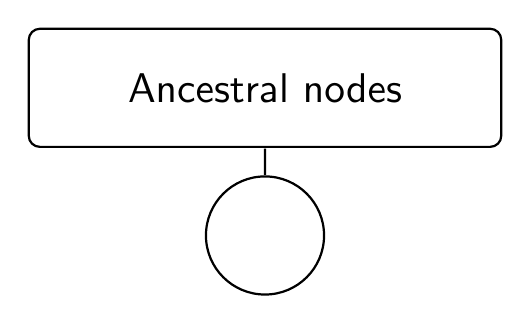
\begin{tikzpicture}[
    scale = 1.5, transform shape, thick,
    every node/.style = {draw, circle, minimum size = 10mm},
    grow = down,  % alignment of characters
    level 1/.style = {sibling distance=3cm},
    level 2/.style = {sibling distance=4cm}, 
    level 3/.style = {sibling distance=2cm}, 
    level distance = 1.25cm
  ]
  \node[shape = rectangle, rounded corners,
    minimum width = 4cm, font = \sffamily] {Ancestral nodes} 
  child { node (Start){}};
  \begin{scope}[nodes = {draw = none}]
    \begin{scope}[nodes = {below = 11pt}]
      \end{scope}
  \end{scope}
\end{tikzpicture}
}
\subfigure{
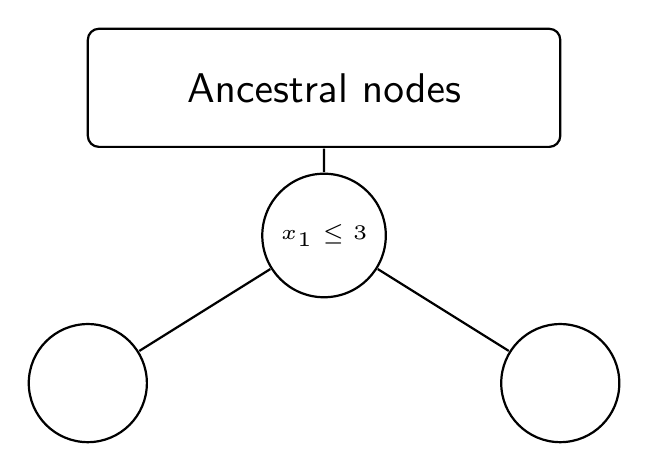
\begin{tikzpicture}[
    scale = 1.5, transform shape, thick,
    every node/.style = {draw, circle, minimum size = 10mm},
    grow = down,  % alignment of characters
    level 1/.style = {sibling distance=3cm},
    level 2/.style = {sibling distance=4cm}, 
    level 3/.style = {sibling distance=2cm}, 
    level distance = 1.25cm
  ]
  \node[shape = rectangle, rounded corners,
    minimum width = 4cm, font = \sffamily] {Ancestral nodes} 
  child { node (Start){\tiny{$x_1 \leq 3$}}
   child {   node (A) {}
       }
   child {   node  (D) {}
     }
  };
  \begin{scope}[nodes = {draw = none}]
    \path (Start) -- (A) node [near start, left]  {};
      \path (Start) -- (D) node [near start, right] {};
    \begin{scope}[nodes = {below = 11pt}]
      \end{scope}
  \end{scope}
\end{tikzpicture}
}
\end{center}
\caption[Illustrating the induction process.]{A terminal node in the decision tree before (left) and after (right) a split on a terminal node.}
\label{fig:induction_firststep}
\end{figure}

The probability measure on the potential splits of the tree is
\begin{equation}\label{eqn:psplit}
p_{\text{split}}(\eta, \mathcal{T})=\alpha(1+d_{\eta})^{-\beta}, \ \ \alpha>0, \beta\geq 0,\\
\end{equation}
where $d_{\eta}$ denotes the depth of the node $\eta$ and $\alpha$, and $\beta$ are scalars. The probability of the specific rule, denoted $\rho$ is 
\begin{equation}\label{eqn:prule}
p_{\text{rule}}(\rho \vert \eta, \mathcal{T}) \propto \underbrace{\Pr(\text{split on covariate})}_{=p_{\text{split}}}\underbrace{\Pr(\text{split on a value given a covariate})}_{=p_{\text{rule}}}. 
\end{equation}

Here CGM recommends using a discrete uniform prior on $p_{\text{split}}$ and splitting uniformly amongst the splitting values (in $p_{\text{rule}}$) that do not result in an empty terminal node. While we choose the same proposal mechanism for the $p_{\text{rule}}$ quantity, the main point of this thesis is to examine and propose alternate specifications for $p_{\text{split}}$. The data sets modeled in CGM \cite{chipman1998bayesian} and DMS \cite{denison1998bayesian}, and other modifications in the literature, deal with data with a small number of predictors. In this thesis we are concerned with a large number of predictors, so we will focus on variable selection, which will ultimately explain how we specify quantity $p_{\text{split}}$ in Equation \ref{eqn:prule}. 

\subsection{Integrated Likelihood}
We will now focus on the integrated likelihood, which is the quantity 

\begin{equation}\label{eqn:int_lhood}
\Pr(Y_i \vert \mathcal{T}, X) = \int_{\Theta}\Pr(Y_i \vert \mathcal{T}_i, X, \theta)\pi(\theta)d\theta.
\end{equation}
To evaluate the integral in Equation \ref{eqn:int_lhood} we must first define a prior, denoted $\pi(\theta)$, for the parameters in each terminal node. 
There are two possible priors for the case of the normal likelihood that will result in a conjugate prior/posterior. These are normal and normals-gamma distributions, or equivalently, normal-inverse gamma distributions depending upon the given parametrization of the scale parameter. 

\subsection{The Process Prior}

Assuming we have a closed form solution for the integral in Equation \ref{eqn:int_lhood}, we can use Bayes' rule to determine 
\begin{equation}\label{eqn:tree_post}
\Pr(\mathcal{T} \vert Y , X) \propto \Pr(Y \vert X ,\mathcal{T})\Pr(\mathcal{T}).
\end{equation} 
We now have an effective means of searching the posterior space over trees to determine the high posterior trees. We can do so by using the Metropolis-Hastings rule 

\begin{equation}\label{eqn:MHrule}
\mathcal{T}^{i+1} =\begin{cases}
\mathcal{T}^*, & \text{with probability}\ \alpha(\mathcal{T}^*, \mathcal{T}^i) = \text{min}\left(\frac{q(\mathcal{T}^*, \mathcal{T}^i)}{q(\mathcal{T}^i, \mathcal{T}^*)}\frac{\Pr(Y\vert X, \mathcal{T}^*)}{\Pr(Y\vert X,\mathcal{T}^i)}\frac{\Pr(\mathcal{T}^{*})}{\Pr(\mathcal{T}^i)},1 \right) \\
\mathcal{T}^{i}, & \text{with probability}\ 1-\alpha(\mathcal{T}^*, \mathcal{T}^i).
\end{cases} \end{equation}

To evaluate the normalization constant would require summing Equation \ref{eqn:tree_post} across all possible trees. This sum includes $\mathcal{O}(nd\frac{4^h}{h^{3/2}})$ terms, with $h$ denoting the maximum height of the trees, $n$ denoting the number of observations, and $d$ denoting the number of covariates. This is an infeasible sum for most data sets, and for all data sets examined in this thesis. For the function $q(-\vert-)$, which is called the proposal function, we use $q$ to propose a new tree $\mathcal{T}^*$.   
In Equation \ref{eqn:MHrule}, $q(\mathcal{T}^*\vert\mathcal{T})$ denotes proposing a new tree $\mathcal{T}^*$, starting from the current tree $\mathcal{T}$. 
 Our proposal mechanism is as follows:
  \begin{itemize}
 \item The grow step chooses at random one of the terminal nodes and proposes to append two new child nodes with a certain probability that could depend on the tree depth, splitting on a chosen covariate.
 \item The prune step works in reverse of the grow. A terminal node is selected at random and that node and the node's sibling are pruned to the immediate parent of the two child nodes.
 \item The change step randomly picks an internal node and attempts to change the split rule at the node with that of another observation, possibly on a different covariate.
  \item The swap step randomly selects an internal node that is not the root node and proposes to swap the split rules of the parent-child pair. If both child nodes split on the same covariate, then both the children and the parent node's rules are swapped.
  \item The rotate step randomly chooses a left or right rotation move. Then this step randomly chooses an admissible internal node and rotates.
 \end{itemize}
  The rotate operation for binary trees was first introduced in Sleater and Tarjan \cite{sleator1985self} and was introduced into Bayesian decision trees in GL \cite{gramacy2008bayesian}. A good introduction and several practical uses of the rotate move can be found in Cormen, Lieserson, Rivest and Stein \cite{cormen2001introduction}. The proposal of Gramacy and Lee \cite{gramacy2008bayesian} only allows a rotate move for the specific case when a swap move is proposed and the parent child pair both split on the same covariate. We modify this rule and allow rotate to be a separate operation of the transition kernel and not a special swap move case. The proposal mechanism of CGM uses the grow, prune, change and swap moves only. We also allow swap moves in our proposal. In addition, neither of CGM nor Gramacy and Lee \cite{gramacy2008bayesian} included weights on each covariate in their examples or model specifications. CGM sampled each covariate and split value uniformly, at random. 
  
 The probability measure on the tree is  
 
 \begin{equation}
 \Pr(\mathcal{T}) = \prod_{\eta \in \mathcal{N}} p_{\text{rule}}(\rho \vert \eta, \mathcal{T})p_{\text{split}}(\eta, \mathcal{T}),
\end{equation}
where $\mathcal{N}$ denotes the set of nodes in tree $\mathcal{T}$.
The probability measure on each split, here denoted $p_{\text{split}}(\eta, \mathcal{T})$, uses Equation \ref{eqn:psplit}. Similarly, the measure on each rule, here denoted $p_{\text{rule}}(\rho \vert \eta, \mathcal{T})$, uses Equation \ref{eqn:prule}. 
All that is left to specify is the likelihood in each node and the prior structure for the parameters in each node, both of which are done in the next subsection. 

\subsection{Node Likelihoods and Priors}

CGM discuss three models. Two of the models use Gaussian priors and Gaussian sampling distribution and one of the models uses a Dirichlet prior and a multinomial sampling distribution. The two Gaussian models differ in that one has a single variance and the other has a different variance for each node. As noted by Lee \cite{lee2006decision}, in a greedy optimization context, sometimes the data suggest a different model than either a Gaussian or a multinomial-Dirichlet. If the experiment suggests analyzing data using an alternate model, the Bayesian context easily handles these alterations, once the corresponding likelihood and prior are specified. Lee \cite{lee2006decision}, proposed a zero inflated poisson (ZIP) model to analyze the solder data. Note our Bayesian model can easily handle extensions such as ZIP response data and also permits covariate selection, provided the integrated likelihood is available in closed form.

We begin with the Gaussian sampling distribution and Gaussian prior model. We define the likelihood as 
\begin{equation}\label{eqn:norm_lhood1}
N[y_{ij} \vert \mu_i, \sigma^2].
\end{equation}
Also, we define the prior for $\mu_i$ as 
\begin{equation}\label{eqn:norm_prior1}
N[\mu_i\vert \bar{\mu}, \sigma^2 ].
\end{equation}
Furthermore, we define the prior for $\sigma^2$ as 
\begin{equation}\newnot{symbol:inv_gamma}
\text{Inv-Gamma}(\sigma^2\vert \alpha, \beta).
\end{equation}
All that remains is to evaluate the integral 
\begin{equation}\label{eqn:int_model1}
\prod_{i=1}^b \int_0^\infty \int_{-\infty}^{\infty} \prod_{j=1}^{n_i} N[y_{ij} \vert \mu_i, \sigma^2]N[\mu_i\vert \bar{\mu}, \sigma^2 ]\text{Inv-Gamma}(\sigma^2\vert \nu/2, \nu\lambda/2)d\mu_id\sigma^2.
\end{equation}
For the Gaussian prior and sampling distribution we can explicitly calculate the marginal likelihood. Being able to marginalize the node parameters explicitly allows us to implement a Metropolis-Hastings algorithm without resorting to complicated, specialized algorithms, or numerical integrations. Straightforward analytic manipulations yield the solution to Equation \ref{eqn:int_model1} written in Equation \ref{eqn:int_model1_soln}
\begin{equation}\label{eqn:int_model1_soln}
\frac{ca^{b/2}}{\prod_{i=1}^b\sqrt{n_i+a}}\times \left(\sum_{i=1}^b\left(\sum_{j=1}^{n_{i}}(y_{ij}-\bar{y}_i)^2\right)+ \frac{(\bar{y}_i -\bar{\mu})^2(n_ia)}{n_i+a} \right)^{-(\nu+n)/2}\hspace{-1.4cm}.
\end{equation}
If we assume instead that the variances might change from node to node, then the stated model is misspecified. Let us denote the variance in each node as $\sigma_i^2$ and keep all other notations from the stated model specification. Then the model is specified using 
\begin{equation}\label{eqn:normal_likelihood_many_variance}
N[y_{ij} \vert \mu_i, \sigma_i^2].
\end{equation}
Also, we define the prior for $\mu_i$ as 
\begin{equation}\label{eqn:multi_variance_prior}
N[\mu_i\vert \bar{\mu}, \sigma_i^2 ].
\end{equation}
Furthermore, we define the prior for the $\sigma_i^2$s as 
\begin{equation}\label{eqn:sigma_priors}
\text{Inv-Gamma}(\sigma_i^2\vert\nu/2, \nu\lambda/2)
\end{equation}
 and now we evaluate the integral equation 
 \begin{equation}\label{eqn:int_model2}
\prod_{i=1}^b \int_0^\infty \int_{-\infty}^{\infty} \prod_{j=1}^{n_i} N[y_{ij} \vert \mu_i, \sigma_i^2]N[\mu_i\vert \bar{\mu}, \sigma_i^2 ]\text{Inv-Gamma}(\sigma_i^2\vert \nu/2, \nu\lambda/2)d\mu_id\sigma_i^2. 
\end{equation}
The result of computing the integrals in Equation \ref{eqn:int_model2} is 
\begin{equation}\label{eqn:int_model3}
\prod_{i=1}^b\pi^{n_i/2}(\lambda\nu)^{\nu/2}\sqrt{\frac{a}{n_i+a}}\frac{\Gamma((n_i+\nu)/2)}{\Gamma(\nu/2)}\times \left( \sum_{j=1}^{n_{i}}(y_{ij}-\bar{y}_i)^2+ \frac{(\bar{y}_i -\bar{\mu})^2(n_ia)}{n_i+a}+\nu\lambda  \right)^{(n_i+\nu)/2}.
\end{equation}
These are the two ``regression'' models for the Bayesian decision trees given in CGM \cite{chipman1998bayesian}. 

The classification model discussed in CGM \cite{chipman1998bayesian} defines the sampling distribution, prior, and integrated likelihood as
\begin{equation}
y_{i1}, \dots, y_{in_i} \vert \mathcal{T} \sim \text{Multinomial}(Y_i \vert \vec{n}, \vec{p}),\newnot{symbol:mult}
\end{equation} 
\begin{equation}
\vec{p} \vert \mathcal{T} \sim \text{Dirichlet}(\vec{p}\vert \vec{\alpha}), \newnot{symbol:dirichlet}
\end{equation} 
and
\begin{equation}\label{eqn:int_model4}
\Pr(Y\vert \mathcal{T}, X)=\left(\frac{\Gamma(\sum_{k=1}^K\alpha_k)}{\prod_{k=1}^K\Gamma(\alpha_k)} \right)^b \prod_{i=1}^b\left( \frac{\prod_{k=1}^K\Gamma(n_{ik}+\alpha_k)}{\Gamma(n_i +\sum_{k=1}^K\alpha_k)} \right),
\end{equation} 
respectively. 
 
If we wanted to model the data using a different data generating process, for example a zero-inflated Poisson, we could do so by specifying a different likelihood, prior, and by computing the integrated likelihood. For a zero-inflated Poisson model defining a likelihood, prior, and calculating the integrated likelihood is possible using gamma priors for the rate ($\lambda$) and beta priors for zero inflation components ($\phi$). 
 
 \subsection{A Bayesian Zero Inflated Poisson Model}
 %\textbf{Write out the details of this model here and cite applied statistics paper which uses a greedy approach.}
 
 Lee and Jin \cite{lee2006decision} reconsidered impurity functions in light of the connection to likelihood functions. Lee and Jin \cite{lee2006decision} proposed to use likelihood functions instead of impurity functions that model the data generating process. Towards this end they considered the soldering data from Chambers and Hastie \cite{chambers1992statistical}. The response of interest in this case is a collection of counts on manufactured circuit boards. This response has many zero values and Lee and Jin \cite{lee2006decision} proposed using a zero inflated (ZIP)\newabbrev{abbrev:ZIP} Poisson likelihood to model the measured counts. Lee and Jin \cite{lee2006decision} optimized using a greedy algorithm and they found the fit and holdout prediction to be better using the ZIP model in each terminal node. If we are to use a Bayesian approach to this problem, we need to define the likelihood, the prior, and the integrated likelihood. We now define these three quantities.
 
 The likelihood for a single observation is 
 \begin{equation}
 f(y\vert \lambda, \phi) \propto \mathds{1}(y=0)\left(\phi + (1-\phi)\exp{(-\lambda)}\right) + \mathds{1}(y>0)\left(\exp{(-\lambda)}\frac{\lambda^y}{y!}\right).
 \end{equation}
 The priors for $\lambda$ and $\phi$ are
 \begin{equation}
 \pi(\phi, \lambda)\propto \underbrace{\frac{\phi^{\alpha-1}(1-\phi)^{\beta-1}\Gamma(\alpha+\beta)}{\Gamma(\alpha)\Gamma(\beta)}}_{=\text{A beta prior }} \times \underbrace{\frac{ \lambda^{\alpha_{\lambda}-1}\exp{(-\lambda/\beta_{\lambda})} }{\Gamma(\alpha_{\lambda})\beta_{\lambda}^{\alpha_{\lambda}}}}_{=\text{A gamma prior}}.
 \end{equation}

 Now we need to calculate the integrated likelihood, which means that we must evaluate 
 \begin{align} \hspace{-.9in}
 &\int_0^1\int_0^\infty \left(\mathds{1}(y=0)\left(\phi + (1-\phi)\exp{(-\lambda)}\right) + \mathds{1}(y>0)\left(\exp{(-\lambda)}\frac{\lambda^y}{y!}\right)\right) \\ \nonumber
 & \frac{\phi^{\alpha-1}(1-\phi)^{\beta-1}\Gamma(\alpha+\beta)}{\Gamma(\alpha)\Gamma(\beta)} \times \frac{ \lambda^{\alpha_{\lambda}-1}\exp{(-\lambda/\beta_{\lambda})} }{\Gamma(\alpha_{\lambda})\beta_{\lambda}^{\alpha_{\lambda}}}d\lambda d\phi.
 \end{align}
 
 Let $j$ index the observed zero counts. Furthermore, let $\bar{y}_{+}$ denote the average of the non-zero counts and $n_0$ and $n_+$ denote the number of zeros and non-zeros in the data respectively. 
 Now we assume that the observations are $i.i.d.$ and simple calculations lead to the conclusion that
 
 \begin{align}\label{eqn:zip_int_lhood}\hspace{-.7in}
 \Pr(Y\vert X, \mathcal{T})& = \left[\sum_{j=0}^{n_0} {n_0 \choose j}\frac{\Gamma(\alpha+\beta)\Gamma(\alpha+j)\Gamma(n_0+\beta-j)}{\Gamma(\alpha)\Gamma(\beta)\Gamma(\alpha+\beta+n_0)}\left(\frac{n_0-j+\beta_{\lambda}^{-1}}{\beta_{\lambda}}\right)^{\alpha_{\lambda}} \right] \\ \nonumber
 & + \frac{\Gamma(\alpha_{\lambda}+n_+\bar{y}_+)}{\Gamma(\alpha_{\lambda})\beta_{\lambda}^{\alpha_{\lambda}}}\left(n_+ + 1/\beta_{\lambda} \right)^{\alpha_{\lambda}+n_+\bar{y}_+}.
\end{align}

A similar calculation may be performed for a response variable that is distributed as a zero-inflated negative binomial random variable (ZINB).\newabbrev{abbrev:ZINB}
 
\section{Previous Variable Selection}
\label{ch:p4sub_var_sel}

Previous approaches to variable selection have focused primarily on the linear model or GLM or GLMM models, all of which we briefly reviewed in Chapter \ref{ch:intro}. Hereafter we will refer to all three types of models as linear. The correspondence between variable selection in linear models and in Bayesian decision trees is a simple correspondence between zeros in the linear model, or zero means of the normal and transformed values on the unit simplex. This correspondence will be detailed in the next subsection of this chapter.   

Ishwaran et al. \cite{ishwaran2010high} propose a modification to Variable Importance (VIMP) criteria that allows some very basic theory to describe the VIMP's analytical properties. VIMP was first proposed by Breiman \cite{breiman2001random} as a method to assess which covariates are important in a dataset. The difficulty with both Ishwaran et al's method and Breiman's method is that they are both very much black box techniques. VIMP basically takes a split in a decision tree on a specific covariate and randomly decides if the observation should go to the left or the right child node. This is done for a collection of observations and the random predictions are averaged against the actual predictions. The resulting numeric estimates for each covariate are the VIMP estimates. A ranking of these values provides a ranking of the covariates. 

A similar method of ranking covariates was proposed by Taddy, Gramacy, and Polson \cite{taddy2011dynamic}. Taddy, Gramacy and Polson proposed a Bayesian approach and used the Bayesian equivalent to $\Delta\phi$ from this chapter, written here for clarity, 
\begin{equation}
\Delta\phi = \int\phi ds - \pi_L\int\phi ds -\pi_R \int \phi_Rds. 
 \end{equation}
Taddy, Gramacy and Polson proposed using samples and estimating the integrals with Monte Carlo approximations. In this case the approach is using a greedy measure on a Bayesian problem, something we find confusing.
In the Bayesian approach the quantity $\Delta\phi$ has little meaning, because we are using an MCMC approach to search across trees. The resulting estimates of the covariates' importance will be the same as the greedy approach, which we find undesirable for many reasons. The method proposed by Taddy, Gramacy, and Polson is worth comparing against our approach because it will have similar difficulties to CGM in high-dimensional data. We will compare their approach to a time series version of our model in future work.
 

 
%\textbf{Write in a brief description of both Ishwaran et al approach and Gramacy and Lee approach}. 

%% previous variable selection details file

\section{Normal Distributions Transformed to the Unit Simplex: The ALoVaS method. }\label{sec:ALN_chapter}

This chapter outlines the additive logistic transformation, which transforms a $d$ dimensional multivariate normal distribution onto the unit simplex in $d+1$ dimensions. Note that the unit simplex in $d+1$ dimensions actually lies in a subspace of $d$ dimensions because of the constraint that the sum of the probabilities equals one. 

The goal of this chapter is to find a transform that moves the space $\mathbb{R}^d$ \newnot{symbol:real} to the simplex $\mathbb{S}^d$. \newnot{symbol:simp} The simplex $\mathbb{S}^d$ is a space defined by the constraints $\{x_i: 0<x_i<1, \sum_{j=1}^dx_j <1 \}$, and the extra term $x_{d+1}=1-\sum_{j=1}^d x_j$ ensures the total sums to 1.  

Define the notation $\yvec$, for the normal random variables that reside in the $\Rsp{d}$  dimensional space. Define the notation $\xvec$  for the vector that resides on $\simp{d}$, the simplex in $d$ dimensions. We use an underline to indicate that the stated quantity is a column vector and capital greek letters (and $I$) will denote matrices (the identity matrix) 

\begin{equation}\label{eqn:simplex_transform}
x_i = \frac{e^{y_i}}{1+\displaystyle{\sum_{j=1}^de^{y_j}}}. \\
\end{equation}
The Jacobian of the transform is defined as
\newnot{symbol:jacobian}
\begin{equation}\label{eqn:jacobian}
J(\yvec \vert \xvec) = \left( \prod_{j=1}^{d+1}x_j \right)^{-1}.
\end{equation}

It is important to note that $\yvec\in\Rsp{d}$, whereas $\xvec\in\simp{d}$. The $d$ dimensional normal has the usual parameters and density

\begin{equation}\label{eqn:multinormal}
f_{\yvec}(\yvec\vert \Sigma, \mu)=(2\pi)^{-d/2}|\Sigma|^{-1/2}\exp{\left(-1/2(\yvec-\muvec)^T\Sigma^{-1}(\yvec-\muvec)\right)}.
\end{equation}

Upon applying the transformation defined by Equation \ref{eqn:simplex_transform}, we arrive at the additive logistic normal (ALN) distribution, with density 

\begin{equation}
f_{\xvec}(\xvec\vert \Sigma, \mu)=\frac{(2\pi)^{-d/2}}{\sqrt{\vert\Sigma\vert}\prod_{j=1}^{d+1}x_j } 
\exp{\left(-1/2(\text{log}(\xvec_{(d+1)}/x_{d+1})-\muvec)^T\Sigma^{-1}(\text{log}(\xvec_{(d+1)}/x_{d+1})-\muvec)\right)}.
\end{equation}
The vector notation $\xvec_{(d+1)}$ denotes the vector in $d$ dimensions that has the $d+1$ entry removed from the vector $\xvec$. 
It is important to note that this density function is defined on the space $\simp{d}$ and \emph{not} on the space $\Rsp{d}$. 

A useful property of this transform is that we can handle probabilities defined on the $d$ dimensional simplex while working with a normal distribution. This is a common and comfortable probability distribution for most statisticians and applied scientists.
We now wish to understand how the specification of the mean vector $\muvec$ and the covariance matrix $\Sigma$ impact the structure of the ALN density. From simulation we can formulate the following conclusions: 

\begin{itemize}
\item With $\Sigma=I$, increasing the mean vector in the positive direction in any one of the $d$ components individually corresponds to shifting density towards the corner of the simplex associated with that covariate. 
\item With $\Sigma=I$, increasing the mean vector in the negative in \emph{all} $d$ components corresponds to shifting density towards the $d+1$ corner of the simplex. 
\item Keeping $\muvec =\vec{0}$, adjusting any of the variances corresponds to shifting towards a projected space of $\simp{d}$. 
\item With $\muvec =\vec{0}$, making one variance small corresponds to the shifting density towards the median of the simplex associated with the remaining $d$ dimensions. 
\item Making the $\Sigma$ matrix approximately singular and moving $\muvec$ in the negative direction for all components places most of the probability density along the median of simplex associated with first $d$ dimensions. 
\item If $\Sigma = \text{Diag}(\sigma^2_j)$,\newnot{symbol:diag} as the $\sigma^2_j$ entries become smaller, the probabilities approach the CGM specification.    
\end{itemize}

Using the transformation defined in Equation \ref{eqn:simplex_transform} and the fact that it is relatively simple to simulate from the vector normal distribution, the ALN density can be simulated. 

\begin{figure}[ht]
\begin{minipage}[b]{0.45\linewidth}
\centering
\includegraphics[width=\textwidth]{mu0_0.pdf}
\caption[ALN plot with a zero mean vector]{In this figure, $\muvec$ has all zero entries, with $\Sigma=I$, corresponding to the equiprobable case. Each probability is approximately $1/(d+1)$. }
\label{fig:figure9}
\end{minipage}
\hspace{0.5cm}
\begin{minipage}[b]{0.45\linewidth}
\centering
\includegraphics[width=\textwidth]{mu-1-1.pdf}
\caption[ALN plot with a negative one mean vector]{In this figure, $\vec{\mu}=(-1,-1)^T$, with $\Sigma=I$, corresponds to moving towards a sparser set of covariates. }
\label{fig:figure10}
\end{minipage}
\end{figure}

\begin{figure}[ht]
\begin{minipage}[b]{0.45\linewidth}
\centering
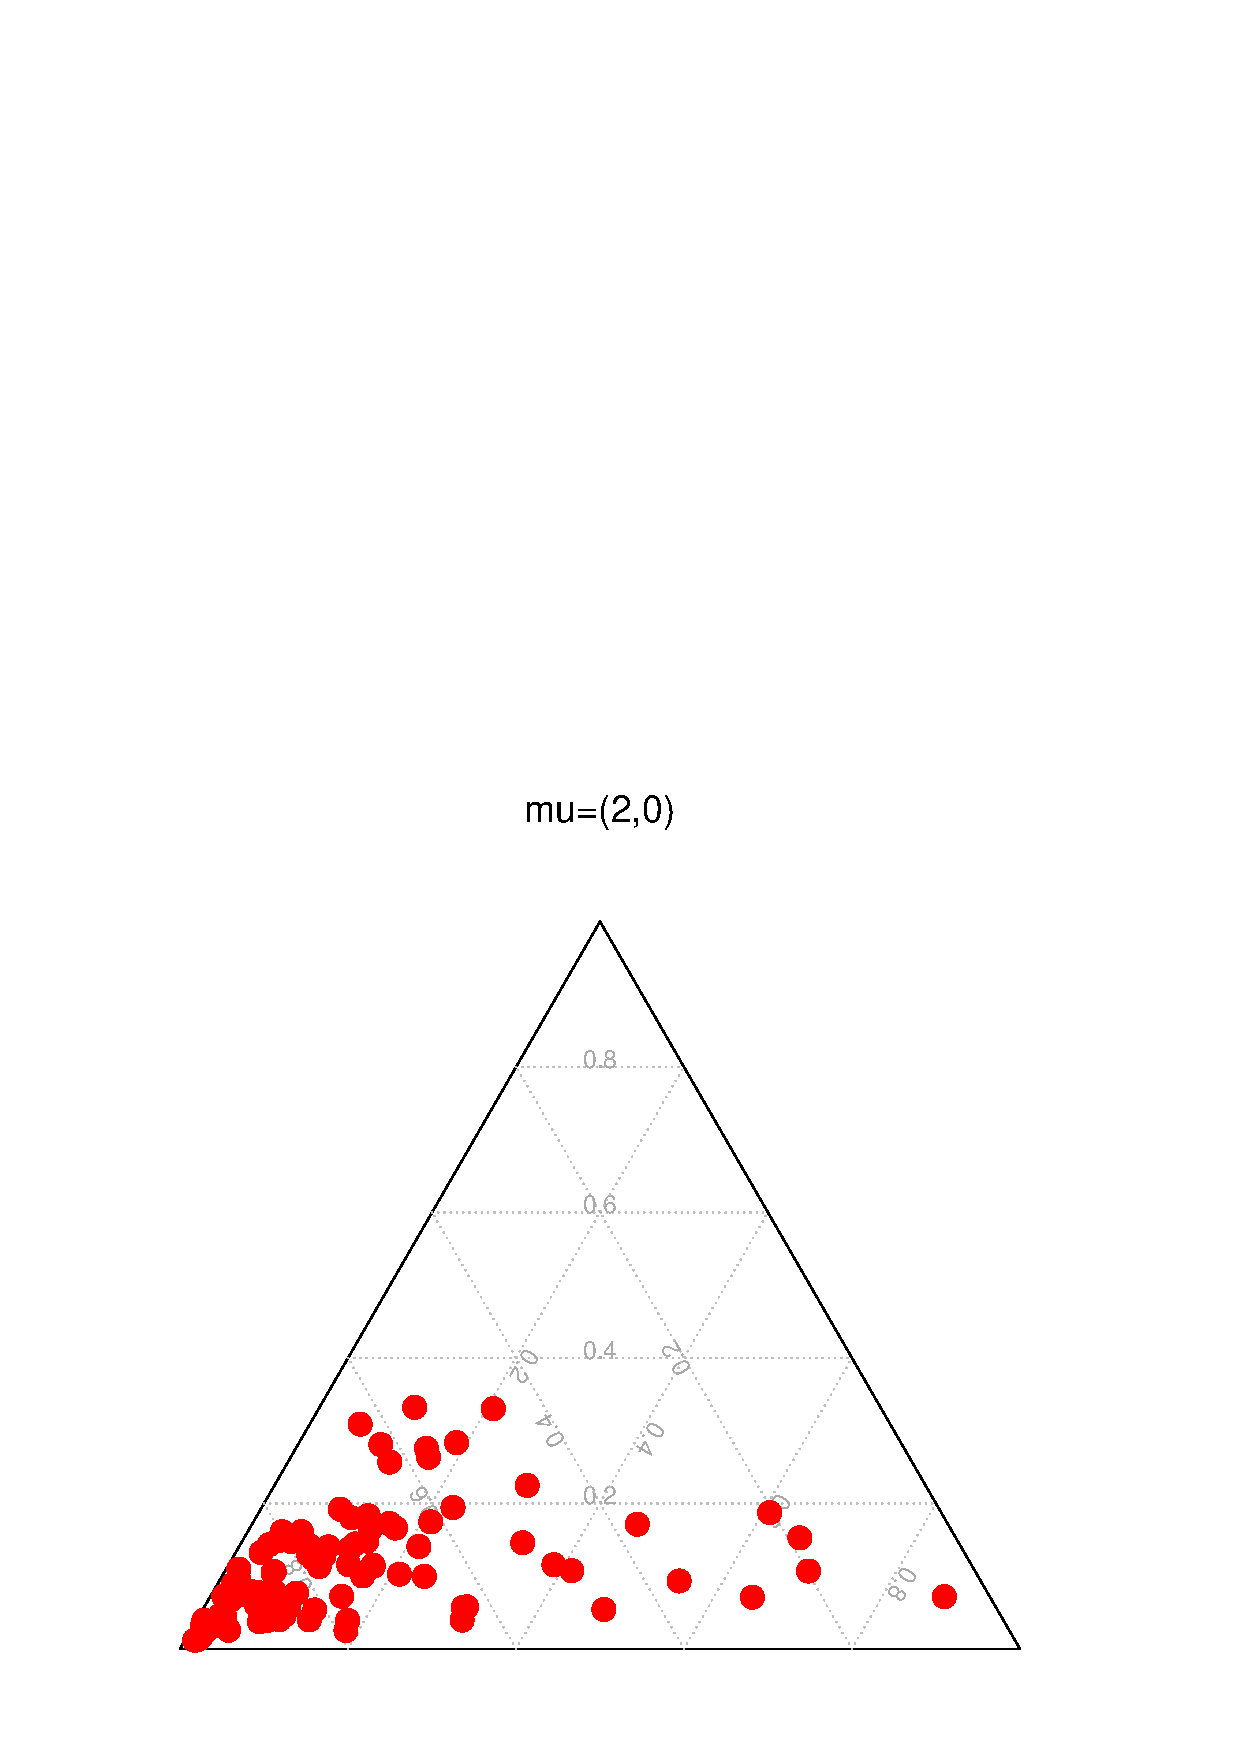
\includegraphics[width=\textwidth]{mu2_0.pdf}
\caption[ALN plot with a mean vector $(2,0)^{T}$]{$\vec{\mu}=(2,0)^T$, with $\Sigma=I$, moves the density towards one corner of the simplex. }
\label{fig:figure1}
\end{minipage}
\hspace{0.5cm}
\begin{minipage}[b]{0.45\linewidth}
\centering
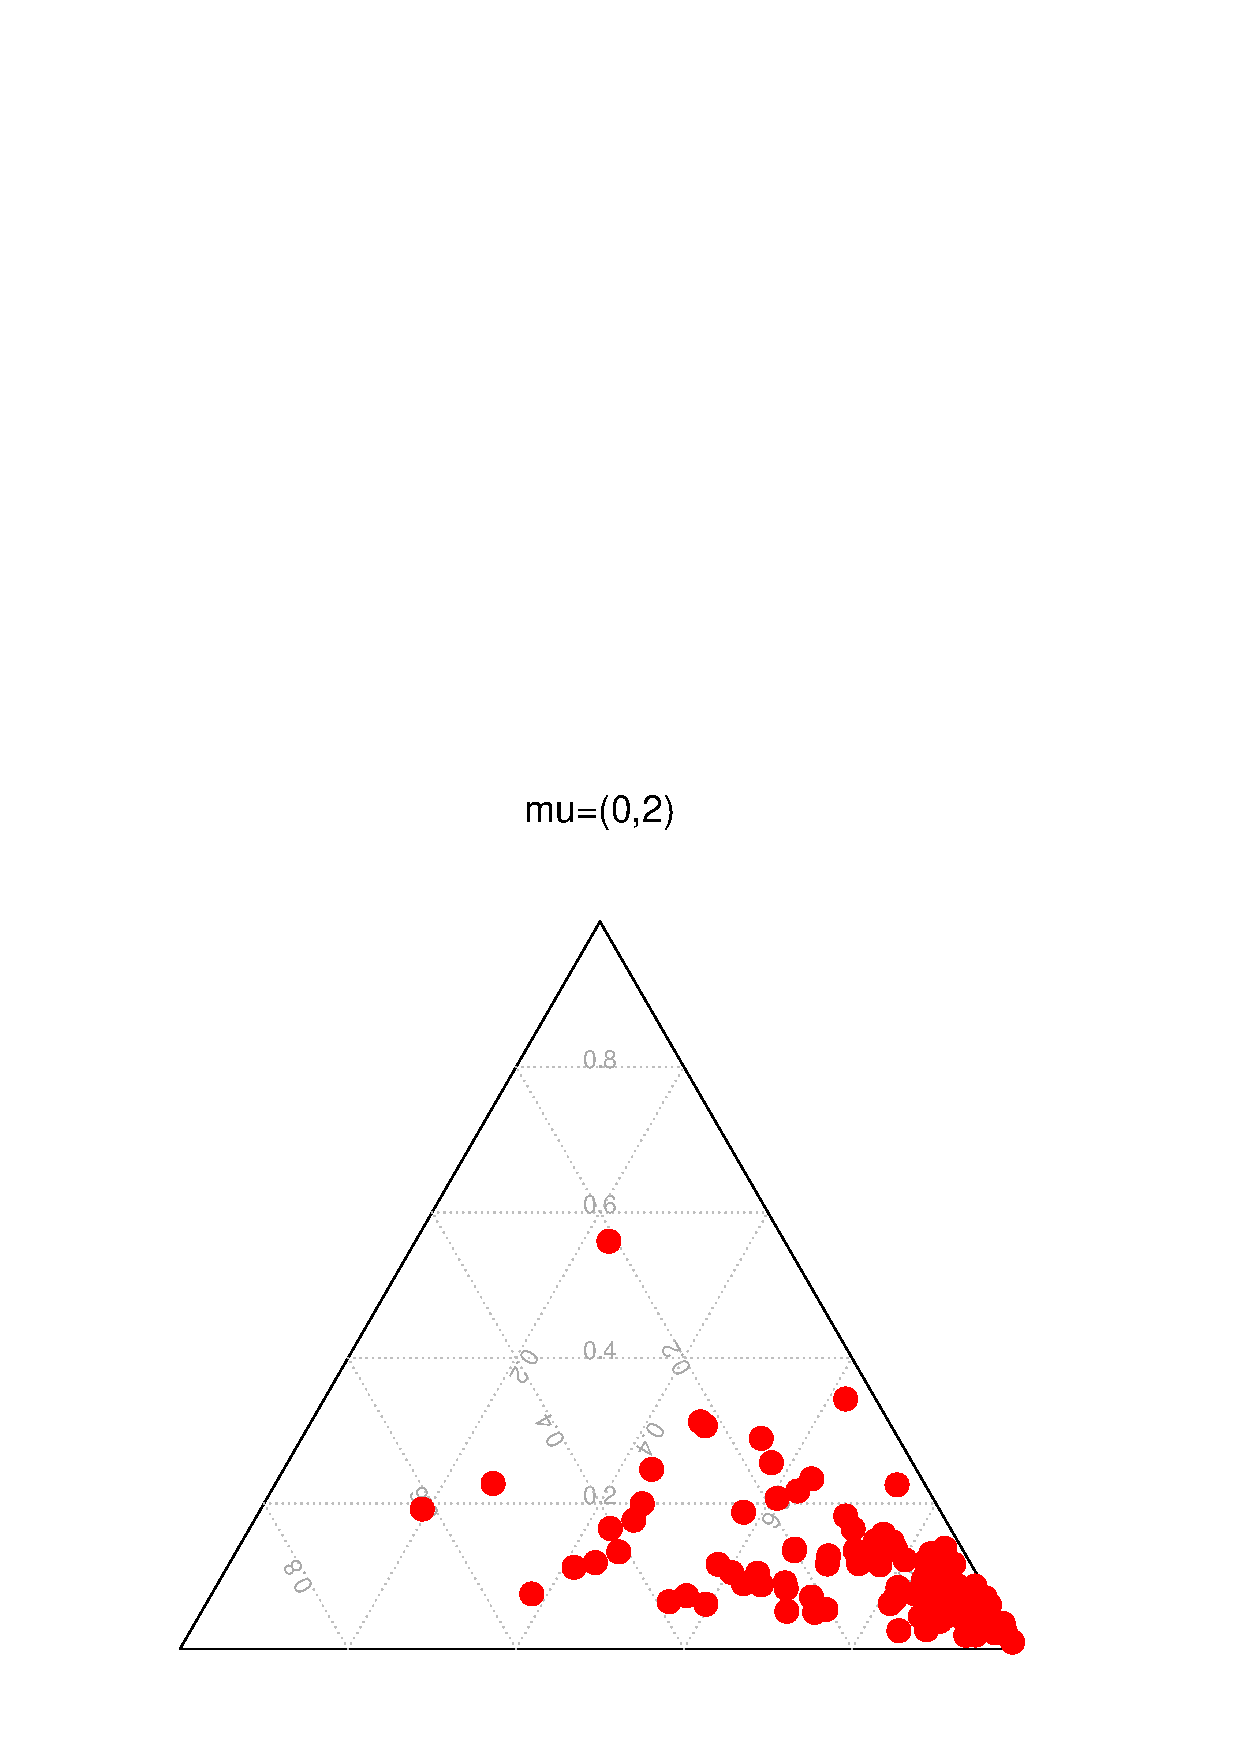
\includegraphics[width=\textwidth]{mu0_2.pdf}
\caption[ALN plot with mean vector $(2,0)^{T}$]{$\vec{\mu}=(0,2)^T$, with $\Sigma=I$, moves the density towards the other corner of the simplex. }
\label{fig:figur2}
\end{minipage}
\end{figure}

\begin{figure}[ht]
\begin{minipage}[b]{0.45\linewidth}
\centering
\includegraphics[width=\textwidth]{mu-2_2.pdf}
\caption[ALN plot with a mean vector of $(-2,2)^{T}$]{$\vec{\mu}=(-2,2)^T$, with $\Sigma=I$, corresponds to most probability mass along a corner of the simplex and is a sparse representation.} 
\label{fig:figure3}
\end{minipage}
\hspace{0.5cm}
\begin{minipage}[b]{0.45\linewidth}
\centering
\includegraphics[width=\textwidth]{Sigma0_01_10.pdf}
\caption[ALN plot $\Sigma=\text{Diag(0.01,100)}$]{ $\vec{\mu}=\vec{0}$, with
 $\Sigma= \text{diag}(0.01, 100)$, corresponds to most density lying on a one dimensional subspace (the second covariate in the $\Rsp\ $ space).  }
\label{fig:figure4}
\end{minipage}
\end{figure}


\begin{figure}[ht]
\begin{minipage}[b]{0.45\linewidth}
\centering
\includegraphics[width=\textwidth]{Sigma1_9_9_1.pdf}
\caption[ALN plot $\Sigma$ numerically singular]{Here $\Sigma$ is approximately singular and most of the probability mass in concentrated along the $d+1$th dimension in the $\mathbb{R}^{d+1}$ space.  }
\label{fig:figure5}
\end{minipage}
\hspace{0.5cm}
\begin{minipage}[b]{0.45\linewidth}
\centering
\includegraphics[width=\textwidth]{Sigma10_0_01.pdf}
\caption[Similar to the case in Figure \ref{fig:figure4} but with the variances reversed]{Similar to the case in Figure \ref{fig:figure4} but with the variances reversed.}
\label{fig:figure6}
\end{minipage}
\end{figure}

 \begin{figure}[ht]
\begin{minipage}[b]{0.45\linewidth}
\centering
\includegraphics[width=\textwidth]{Sigma100_100.pdf}
\caption[ALN plot with a zero vector mean and $\Sigma=\text{Diag}(100,100)$]{$\vec{\mu}=\vec{0}$, with
 $\Sigma= \text{diag}(100, 100)$, corresponds to encouraging sparse representations \emph{a priori}.  }
\label{fig:figure7}
\end{minipage}
\hspace{0.5cm}
\begin{minipage}[b]{0.45\linewidth}
\centering
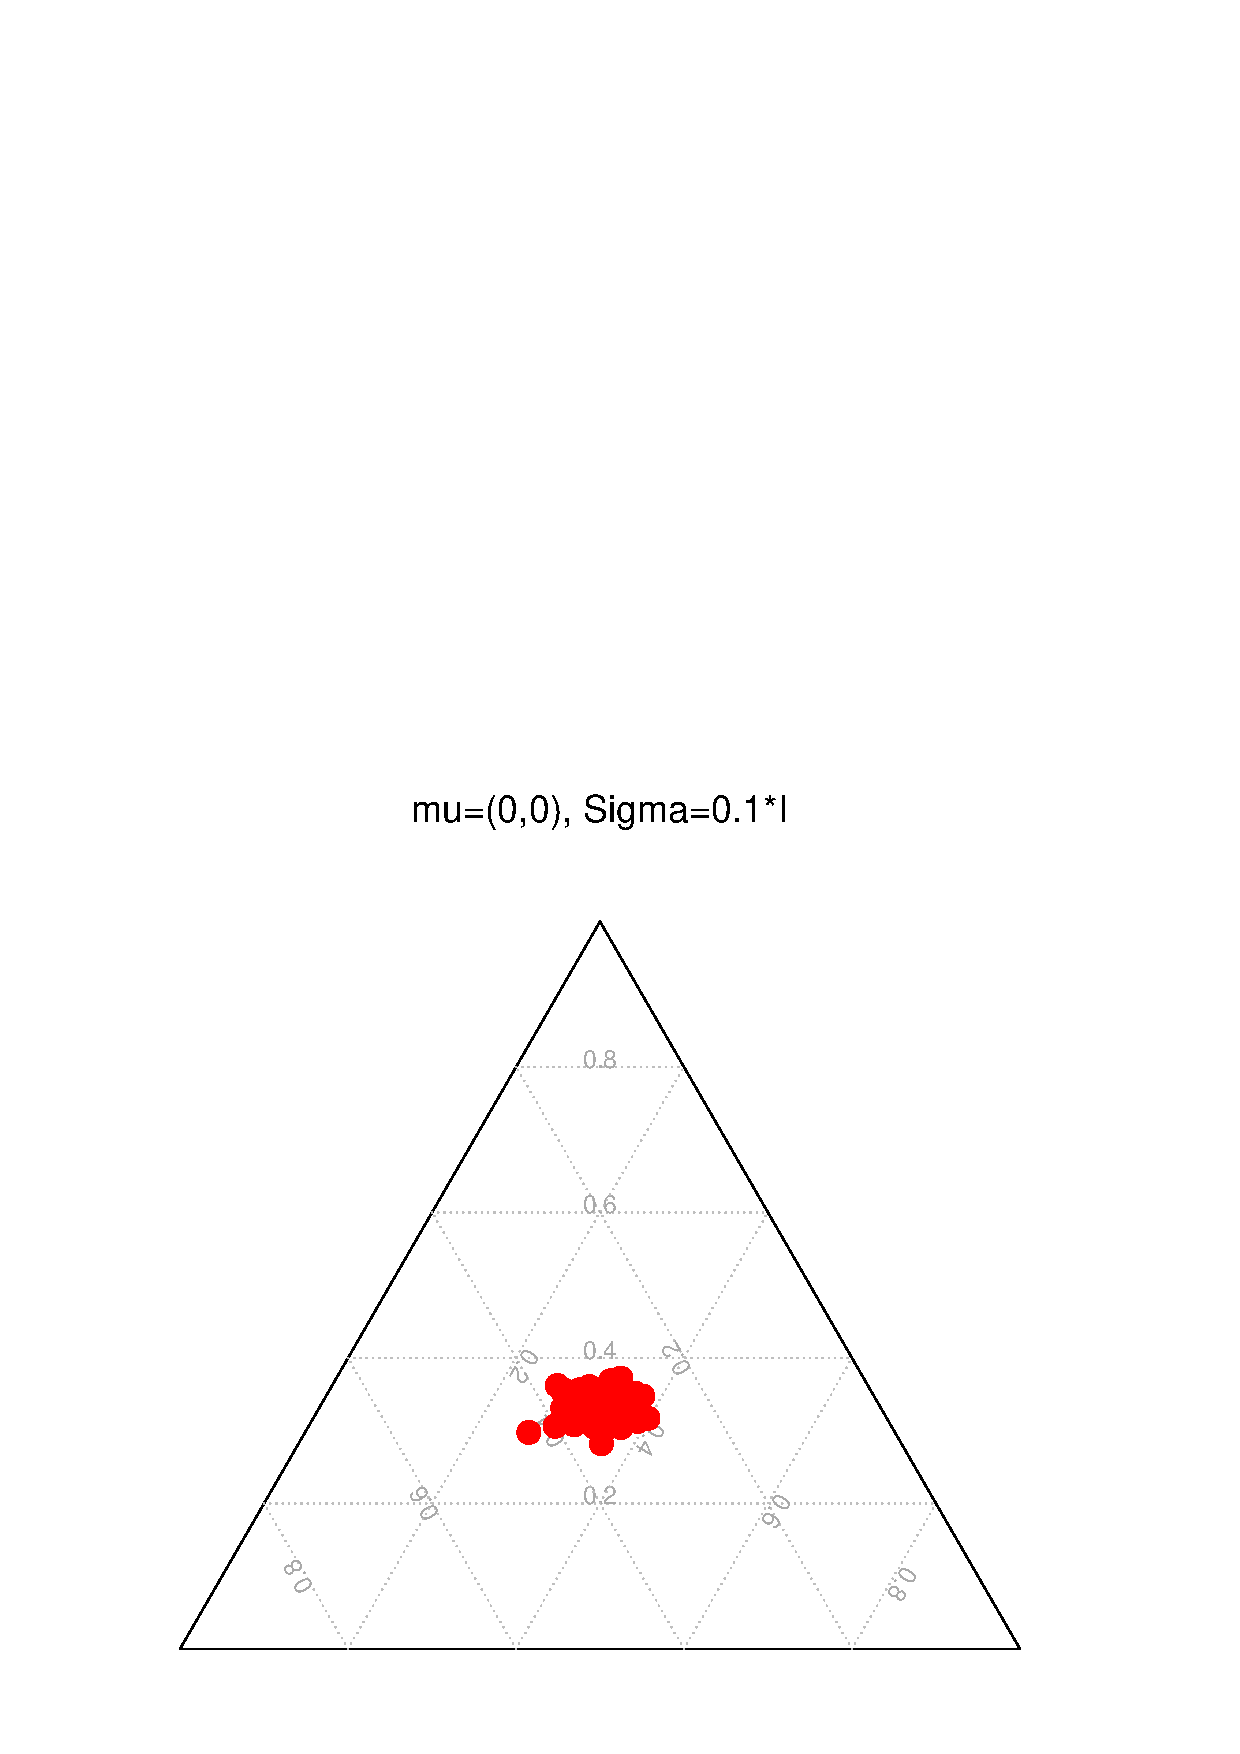
\includegraphics[width=\textwidth]{Sigma01_01.pdf}
\caption[ALN plot approximating the CGM model]{Here $\Sigma=0.1I$, and $\muvec=\vec{0}$, corresponds to roughly the CGM specification.}
\label{fig:figure8}
\end{minipage}
\end{figure}

 The simulations indicate that we can scale everything at approximately an $\mathcal{O}(d)$\newnot{symbol:big_oh} rate because of the diagonality of the variance covariance matrix, no matrix inversions are required. The step that remains is to link this portion of the model with the (currently) observed data in the tree, so that better trees are favored over trees that are worse, when each is observed in the Markov chain. We will first work in the space $\Rsp{d}$ and then translate to probabilities by using Equation \ref{eqn:simplex_transform}.  
 
 If we are to focus on the means and a collection of variances in a multivariate normal i.i.d. model, then we must fully specify the likelihood and the prior to form our posterior. 
 
 The likelihood of the tree is defined as follows: the tree's selected covariates are counted and summed across all observed splits, leading to a likelihood taking on discrete values for the observed data. Let us define a multiplier that can take on an arbitrary positive or negative value in a compact region. We then multiply the counts of splits on each covariate by this quantity, effectively creating a mean which can take on arbitrary values in $\Rsp{}$. 

\subsection{A Simple Sampler Approach}

This subsection derives the full conditional densities for each necessary update in the Gibbs loop to sample posterior weights on each dimension in the CGM decision tree sampler. 
 Throughout this subsection we will use the notation $\odot$\newnot{symbol:hadamard} to denote a Hadamard product of two matrices or vectors. 
 
 \subsubsection{The General Strategy}
 There are many problems with using a Dirichlet prior and a Multinomial conjugate likelihood. The two most glaring problems are the implicit prior assumption of same scales on each covariate and the fact that all covariances or, equivalently, correlations must be negative. If the generative model of the data is a linear model with an interaction term and a decision tree model is fit to the data, then several splits will occur on the two interacting covariates. These splits will occur alternately until the curvature is sufficiently approximated \cite{ishwaran2010high}. This situation indicates a positive correlation between the two covariates. Higher order interactions will result in similar positive correlations between collections of covariates. Therefore we conclude the Dirichlet density as a posterior for the probability of selecting a covariate is an inferior model. Moreover, the initial motivation for modeling data with a decision tree was to handle survey data that contained many complex interactions that would be too computationally expensive to evaluate using linear model methods \cite{morgan1963problems}. 
 
 The likelihood will be denoted by
 
 \begin{equation}\newnot{symbol:mvn}
 MVN(\vec{c}\odot\vec{s}\vert \vec{\mu}, \Sigma=\text{Diag}(\sigma^2_j)).
 \end{equation}
 
 The prior is also a normal 
 
 \begin{equation}
 \pi(\vec{\mu}\vert \vec{\mu}_p, \Sigma)=MVN(\vec{\mu}\vert \vec{\mu}_p, \Sigma).
 \end{equation}

The priors on the variances are \iid $\sim \invgam{\sigma_j^2}{a_j}{b_j}$.
Finally the priors on the $c_j$s are \iid\ scaled beta's with densities 

\begin{equation}\newnot{symbol:scaled_beta}
S\beta(c_j\vert \alpha_j, \beta_j, -a, a)\equiv\pi(c_j\vert \alpha_j, \beta_j, -a, a)= \frac{(c_j+a)^{\alpha_j-1}(a-c_j)^{\beta_j-1}\Gamma(\alpha_j+\beta_j)}{(2a)^{\alpha_j+\beta_j-1}\Gamma(\alpha_j)\Gamma(\beta_j)}.
\end{equation}

A special case of these scaled beta densities is when $\alpha_j=\beta_j=1$, which yields uniform r.v.'s on the region  $[-a,a]$. 
For each $j=1, \dots, d$, we first calculate $s_j = \epsilon+\sum_{\forall \eta \in \mathcal{T}}\mathds{1}[\text{split on covariate j at node $\eta$}]$, for some fixed $\epsilon>0$.
Through basic Bayesian calculations we find that the full conditionals are 

\begin{equation}
\pi(c_j\vert \mu_j, \sigma_j^2, a) \sim N_{[-a,a]}(c_js_j\vert \mu_j, \sigma^2_j) \text{(a normal truncated to the region $(-a,a)$),}
\end{equation}

\begin{equation}
\pi(\sigma^2_j \vert \mu_j, c_j, a) \sim \invgam{\sigma_j^2}{2a_j+2}{\frac{(c_js_j-\mu_j)^2+ (\mu_j-\mu_j^p)^2+b_j}{2}}, \text{ and } 
\end{equation}

\begin{equation}
\pi(\mu_j\vert \mu_j^p, c_j, \sigma^2_j)\sim N[c_js_j+\mu_j^p, \sigma_j^2].
\end{equation}

Ideally we would like everything to be a Gibbs step. This can be accomplished numerically using numerical approximations to the cumulative density of the standard normal distribution, here denoted $\Phi$, and $\Phi^{-1}$, the quantile function of the standard normal cumulative density. \newnot{symbol:sncdf} However, we can accomplish this directly using the technique of parameter expansion set forth in Damien and Walker \cite{damien2001sampling}, which we review here for completeness. 
 
We begin with the joint density of two random variables 

\begin{equation}
f(x,y) \propto \mathds{1}[0, \exp{(-x^2/2)}](y).
\end{equation}
The marginal of $x$ is a standard normal density. Through elementary probability calculations we find 

\begin{equation}\newnot{symbol:unif}
f(y\vert X=x) \propto Unif(0, \exp{(-x^2/2)}).
\end{equation}
 and 
 
 \begin{equation}
f(x\vert Y=y) \propto Unif(-\sqrt{-2log(y)}, \sqrt{-2log(y)})
\end{equation}
 The region upon which $X$ is defined arises from the solution of the inequalities $\{0\leq y \leq \exp{(-x^2/2)} \} $ for $X$, which is a quadratic equation in $X$. Similarly, if we have a truncated distribution truncated to the region $[a,b]$, we write the joint density 
 
 \begin{equation}
 f(x,y)=Unif((0\leq y\leq \exp{(-x^2/2)})\times (a,b)).
 \end{equation}
 Solving the resulting system of inequalities leads to the set 
 
 \begin{equation}
 \{-\sqrt{-2log(y)}, \sqrt{-2log(y)} \} \cap \{a, b\},
 \end{equation}
which results in the region for $x$

\begin{equation}
 \{\text{max}(a,-\sqrt{-2log(y)}), \text{min}(b,\sqrt{-2log(y)} )\} .
 \end{equation}
 Simulating from a truncated normal is equivalent to simulating from two uniforms on the appropriate regions and evaluating a natural logarithm and a square root. 
 
 A special case of these scaled beta densities is when $\alpha_j=\beta_j=1$, which yields uniform random variables on the region $[-a,a]$. 
For each $j=1, \dots, d$, we first calculate $s_j = \epsilon+\sum_{\forall \eta \in \mathcal{T}}\mathds{1}[\text{split on covariate j at node $\eta$}]$, for some fixed $\epsilon>0$.
Through basic Bayesian calculations we find the full conditionals in closed form
 
\begin{equation}\label{eqn:u_given_cjsj}
\pi(u \vert c_js_j, \mu_j, \sigma_j^2)= \text{Unif}(0, \exp{(\frac{-(c_js_j-\mu_j)^2}{2\sigma_j^2} )}),
\end{equation}

\begin{equation}
\pi(c_j \vert u) = \text{Unif}(\text{max}(-a,-\sqrt{-2log(u)}), \text{min}(a,\sqrt{-2log(u)} )),
\end{equation}

\begin{equation}
\pi(\sigma^2_j \vert \mu_j, c_j, a) \sim \invgam{\sigma_j^2}{2a_j+2}{\frac{(c_js_j-\mu_j)^2+ (\mu_j-\mu_j^p)^2+b_j}{2}}, \text{ and}
\end{equation}

\begin{equation}\label{eqn:muj_given_cj}
\pi(\mu_j\vert \mu_j^p, c_j, \sigma^2_j)\sim N[c_js_j+\mu_j^p, \sigma_j^2].
\end{equation}

 The Gibbs sampling step, nested within the MH sampler, proceeds by sampling from Equations \ref{eqn:u_given_cjsj}-\ref{eqn:muj_given_cj}
At each iteration, once samples are drawn in sequence from the distributions given in Equations \ref{eqn:u_given_cjsj}- \ref{eqn:muj_given_cj}, we take the posterior samples of $\mu_j$ and transform these onto the $[0,1]$ scale, by using the ALN transform given in Equation \ref{eqn:simplex_transform}. 

We show results from a preliminary coding of the stated algorithm. We use two specificications for the prior means $\vec{\mu}^p$. One specification uses  $\vec{\mu}^p = \vec{0}$ (Figure \ref{fig:simple_sampler2}) and another uses $\vec{\mu}^p=(-2,-2,2,\dots,2)$ (Figure \ref{fig:simple_sampler1}). The difference in the results of sampled weights indicates that, if we can move from a negative to a positive value for the prior mean, we can greatly influence the selection of covariates. The graphic of posterior weights shown in Figure \ref{fig:simple_sampler1} is the correct set of weights for the data. 


%%%% -------Graphics from preliminary simulations using the simple sampler approach

 \begin{figure}[ht]
\begin{minipage}[b]{0.45\linewidth}
\centering
\includegraphics[scale=0.4]{simple_sampler2.png}
\caption[Results for the zero mean prior]{A zero mean prior. Note that the two covariates that should have large probabilities are covariates 1 and 2.}
\label{fig:simple_sampler2}
\end{minipage}
\hspace{0.5cm}
\begin{minipage}[b]{0.45\linewidth}
\centering
\includegraphics[scale=0.4]{simple_sampler1.png}
\caption[Results for the informative prior]{An informative prior. The first two prior means are 2 and the remaining prior means are set at -2.}
\label{fig:simple_sampler1}
\end{minipage}
\end{figure}


%%%%---------END OF: Graphics from preliminary simulations using the simple sampler approach


%\subsection{An Inverse Wishart Prior}
%
%The next generalization is to proceed via an Inverse Wishart prior approach. 
%
%\subsection{A Multivariate Half Cauchy Prior for $\Sigma$}
%
%Using the results of the Bayesian Analysis paper of Huang and Wand \cite{huang2013simple} we can provide a marginally non informative prior on $\Sigma$ which encourages sparsity.  
%
%\subsection{A Stochastic Search Variable Selection Approach}
%
%Using the results of George and McCulloch we can derive Gibbs updates for each of the parameters and have as a special case the approach of CGM if all the dimension indicators are selected to be the point masses at zero. In this case the ALN transform puts probability $1/(d+1)$ on each dimension. 
%
%Include Geweke's Modification and Mitchell and Beauchamp


\section{Derivations}
\label{ch:p3sub_theory}

This subsection contains the mathematical details for calculating the integrals to get the closed form solutions for the integrated likelihood equations of the ZIP model described in this chapter.   

%\subsubsection{Normal Derivation}

\subsection{ZIP Derivations}

In this section we provide the derivation for the integrated likelihood for the Bayes ZIP (zero inflated Poisson) tree model. Now let us define our notation, $j$ will index all observations or only the observed zero observations with the upper limit being $n$ or  $n_0$ if the index is all observations or observed zero counts only, respectively.  Also $j^{\prime}$ will exclusively index the non-zero observations. The total number of non-zero observations is denoted $n_+$, so that $n_++n_0=n$, the total number of observations. Finally, let $\bar{y}_{i+}$ denote the sample mean of the non-zero count observations in terminal node $i$. 

The integrated likelihood is:
\begin{align*}
\Pr(Y \vert X, \mathcal{T}) &= \prod_{i=1}^b\int_0^1\int_0^\infty\prod_{j=1}^{n_i}\left[\mathds{1}[y_{ij}=0](\phi+(1-\phi)\exp{(-\lambda)})+\mathds{1}[y_{ij}>0]\frac{\exp{(-\lambda)\lambda^{y_{ij}}}}{y_{ij}!} \right]\pi(\phi_i,\lambda_i )d\lambda_id\phi_i\\
&=\prod_{i=1}^b \int_0^1\int_0^\infty\underbrace{\prod_{j=1}^{n_0}(\phi + (1-\phi)\exp{(-\lambda)})\pi(\phi_i,\lambda_i )d\lambda_id\phi_i}_{=(1)}\\ 
&+ \prod_{i=1}^b \int_0^1\int_0^\infty \underbrace{\prod_{j^\prime=1}^{n_+}\frac{\exp{(-\lambda)}\lambda^{y_{ij^\prime}} }{y_{ij^\prime}!}\pi(\phi_i,\lambda_i )d\lambda_id\phi_i}_{=(2)}.\\ 
\end{align*} 
We will first tackle $(1)$, then $(2)$. 

\begin{align*}
(1)&= \int_0^1\int_0^\infty\prod_{j=1}^{n_0}(\phi + (1-\phi)\exp{(-\lambda)})\pi(\phi_i,\lambda_i )d\lambda_id\phi_i \\
&= \int_0^1\int_0^\infty(\phi + (1-\phi)\exp{(-\lambda)})^{n_0}\pi(\phi_i,\lambda_i )d\lambda_id\phi_i \\
&= \int_0^1\int_0^\infty\sum_{j=1}^{n_0}{n_0\choose j}\phi^{j}(1-\phi)^{n_0-j}\exp{(-(n_0-j)\lambda)})\pi(\phi_i)\pi(\lambda_i )d\lambda_id\phi_i. \\
\end{align*}
Now, we take $\pi(\phi_i)$ to be a beta($\alpha, \beta$) prior and $\pi(\lambda_i)$ to be a gamma($\alpha_{\lambda}, \beta_{\lambda}$) prior. This simplifies matters greatly. The last equation above with a double integral becomes:
 \begin{align*}
 & \int_0^1\int_0^\infty\sum_{j=1}^{n_0}{n_0\choose j}\phi^{j}(1-\phi)^{n_0-j}\exp{(-(n_0-j)\lambda)})\frac{\Gamma(\alpha+\beta)\phi^{\alpha-1}(1-\phi)^{\beta-1}}{\Gamma(\alpha)\Gamma(\beta)}\frac{\lambda^{\alpha_{\lambda}-1}\exp{(-\lambda/\beta_{\lambda})}}{\Gamma(\alpha_{\lambda})\beta_{\lambda}^{\alpha_{\lambda}}} d\lambda_id\phi_i \\
&=\sum_{j=1}^{n_0}{n_0\choose j}\frac{\Gamma(\alpha+\beta)}{\Gamma(\alpha)\Gamma(\beta)\Gamma(\alpha_{\lambda})\beta_{\lambda}^{\alpha_{\lambda}}} \underbrace{\int_0^1\phi^{j+\alpha-1}(1-\phi)^{\beta+n_0-j-1}d\phi_i}_{\text{a beta kernel}}  \underbrace{\int_0^\infty \lambda^{\alpha_{\lambda}-1} \exp{(-(n_0-j+\beta_{\lambda}^{-1})\lambda)} d\lambda_i}_{\text{a gamma kernel}}\\
&=\underbrace{\sum_{j=1}^{n_0}{n_0\choose j}\frac{\Gamma(\alpha+\beta)}{\Gamma(\alpha)\Gamma(\beta)\Gamma(\alpha_{\lambda})\beta_{\lambda}^{\alpha_{\lambda}}} \frac{\Gamma(\alpha+j)\Gamma(\beta+n_0-j)\Gamma(\alpha_{\lambda})}{\Gamma(\alpha+\beta+n_0)}(n_0-j+\beta_{\lambda}^{-1})^{\alpha_{\lambda}}}_{=(1)}.
\end{align*} 
Now with the first piece simplified, we move on to piece $(2)$. 
 
 \begin{align*}
 (2) &= \int_0^1\int_0^\infty\prod_{j^\prime=1}^{n_+}\frac{\exp{(-\lambda)}\lambda^{y_{ij^\prime}} }{y_{ij^\prime}!}\pi(\phi_i,\lambda_i )d\lambda_id\phi_i \\
 &= \int_0^\infty \prod_{j^\prime=1}^{n_+}\frac{\exp{(-\lambda)}\lambda^{y_{ij^\prime}} }{y_{ij^\prime}!}\pi(\lambda_i )d\lambda_i \\
 &= \int_0^\infty\frac{\exp{(-n_+\lambda)}\lambda^{n_+\bar{y}_{i+}} }{\prod_{j^\prime=1}^{n_+}y_{ij^\prime}!}\pi(\lambda_i )d\lambda_i \\
 &= \int_0^\infty\frac{\exp{(-n_+\lambda)}\lambda^{n_+\bar{y}_{i+}} }{\prod_{j^\prime=1}^{n_+}y_{ij^\prime}!}\frac{\lambda^{\alpha_{\lambda}-1}\exp{(-\lambda/\beta_{\lambda})}}{\Gamma(\alpha_{\lambda})\beta^{\alpha_{\lambda}}_{\lambda}}d\lambda_i \\
 &= \frac{\int_0^\infty\exp{(-(n_+ +\beta_{\lambda}^{-1})\lambda)}\lambda^{n_+\bar{y}_{i+} +\alpha_{\lambda}-1} d\lambda_i}{\Gamma(\alpha_{\lambda})\prod_{j^\prime=1}^{n_+}y_{ij^\prime}!\beta^{\alpha_{\lambda}}_{\lambda}} \\
 &= \underbrace{\frac{\Gamma(n_+\bar{y}_{i+}+\alpha_{\lambda})(n_+ +\beta_{\lambda}^{-1})^{n_+\bar{y}_{i+}+\alpha_{\lambda}}}{\Gamma(\alpha_{\lambda})\prod_{j^\prime=1}^{n_+}y_{ij^\prime}!\beta^{\alpha_{\lambda}}_{\lambda}}}_{=(2)}. \\
 \end{align*}
This is the result we need, putting the two parts together gives the closed form for the integrated likelihood. We rewrite Equation \ref{eqn:zip_int_lhood} here for completeness, 

\begin{align}\nonumber
 \Pr(Y\vert X, \mathcal{T})& = \left[\sum_{j=0}^{n_0} {n_0 \choose j}\frac{\Gamma(\alpha+\beta)\Gamma(\alpha+j)\Gamma(n_0+\beta-j)}{\Gamma(\alpha)\Gamma(\beta)\Gamma(\alpha+\beta+n_0)}\left(\frac{n_0-j+\beta_{\lambda}^{-1}}{\beta_{\lambda}}\right)^{\alpha_{\lambda}} \right] \\ \nonumber
 & + \frac{\Gamma(\alpha_{\lambda}+n_+\bar{y}_+)}{\Gamma(\alpha_{\lambda})\beta_{\lambda}^{\alpha_{\lambda}}}\left(n_+ + 1/\beta_{\lambda} \right)^{\alpha_{\lambda}+n_+\bar{y}_+}.
\end{align}
The reader should now clearly see the first and second quantities from the derivations above in succession in the above equation. While the number of observed zeros, $n_0$, is small this finite sum can easily be calculated. For a large dataset, perhaps with a large number of zeros, a numeric approximation may be sufficient for practical implementation.

The reader should understand that for efficient sampling terminal node models beyond the common normal and Dirichlet terminal node models. Bayesian decision trees with counts as a response, including counts with an excess of zeros, and over dispersed can easily be handled. The only difficulty might lie in the numeric evaluation of the series in the zero-inflated terminal node models. However, this should not be too much of an issue because Sterling's approximation to the Gamma can be applied with good accuracy in most settings. Moreover, should the number of observed zeros, $n_0$ be too large an integral approximation to the sum should suffice. 
\newpage

\chapter{Bayesian Decision Tree Models}\label{sec:Model}

In Sections \ref{sec:lhood} and \ref{subsec:alt} we describe how we use the ALT to link sparse linear models with covariate selection probabilities facilitating sparse Bayesian decision trees. In Section \ref{subsec:the_tp} we describe the tree prior and the local updates we use to explore the graph of permissible trees. %Finally, in Section \ref{subsec:Regularization Priors} we give several examples of regularization priors we will study in our simulated examples.

	\section{The Likelihood}\label{sec:lhood}

We begin by reviewing the model proposed in Chipman et al. \cite{chipman1998bayesian}, and show how our approaches generalize upon their model. 

The response data is usually assumed to be observed from a normal or multinomial likelihood function. Nonetheless, other forms of response data such as zero inflated models are possible \cite{lee2006decision}. The likelihood is denoted 

\begin{equation}\label{eqn:cgm_likelihood}
\mathcal{L}(\mathcal{T}, \vec{q}, \vec{\theta} \vert \vec{y} X)=\Pr(\vec{y} \vert X, \mathcal{T}, \vec{q}, \vec{\theta}).
\end{equation} 
		
\noindent Here the $\vec{y}$ denotes the vector of responses, $X$ denotes the matrix of covariates, and $\mathcal{T}$ denotes the tree. The vector $\vec{q}$ is the vector of covariate selection probabilities and $\vec{\theta}$ denotes the vector of parameters in the terminal nodes of the tree. The parameters that we are interested in are: $\mathcal{T}$, $\vec{\theta}$, and $\vec{q}$. We factorize the prior in a similar fashion to Chipman et al. using the breakdown 

\begin{equation}\label{eqn:prior}
\Pr(\mathcal{T}, \vec{q}, \vec{\theta}) \propto \Pr(\vec{\theta} \vert \mathcal{T}) \Pr(\vec{q} \vert \mathcal{T})\Pr(\mathcal{T}).
\end{equation} 

The framework in Chipman et al. \cite{chipman1998bayesian} proposed assumed $\vec{q} \propto 1/p$. Although we find this prior to be a strong \emph{a priori} assumption to take with a large dimensional covariate space, this prior will be seen as a special case of the SSVS prior presented in Section \ref{sec:ALoVaS_model}. Practical difficulties with the uniform prior were already noted in the discussion of Chipman et al. \cite{knight1998bayesian}, although, little work has been done in the interim to remedy this drawback. We modify the framework of Chipman et al. to allow the $\vec{q}$ to vary, depending on their relevance. We specify a prior on the $\mu_j$, a linear space, and use the \ALT\ to determine (indirectly) the prior on the probability space of the $\vec{q}$. This prior specification on the $\mu_j$ allows one to use the methods of the sparse linear model literature but instead apply these methods to decision trees. 

The prior density for $\vec{q}$, the covariate selection probabilities, is defined in Subsection \ref{subsec:alt}. Similar to Chipman et al., we place the uniform prior, denoted $\Pr(\mathcal{T})$, on the decision tree space. We sample the decision trees using the stochastic process defined in Section \ref{subsec:the_tp}.  To monitor the convergence of the Markov chain used to sample the space of decision trees, it is necessary to be able to calculate the marginal density for $\mathcal{T}$ given the covariate selection probabilities $\vec{q}$. This requires choosing conjugate priors for the vector $\vec{\theta}$ so that a closed form marginal density, $\Pr(\vec{y}\vert X,\vec{q},\mathcal{T})$ is available. Thus, if the response data are continuous, we choose a Gaussian density for the prior on $\vec{\theta}$. Similarly, if the response data are categorical, we choose a Dirichlet density as the prior density for $\vec{\theta}$.  

	\section{The Additive Logistic Transform}\label{subsec:alt}
	
	The ALT, defined in Equation \ref{eqn:alt}, is a mapping from a Euclidean space to a probability space. 
	%We define our model on a Euclidean space and then, once the draw from the posterior is simulated, we transform the draw to a probability scale using the ALT. 
	The ALT was proposed previously as a fundamental transform for use in compositional data analysis \cite{aitchison1986statistical}. 
	
	The additive logistic normal (ALN) density is obtained as a result of transforming a multivariate normal density using the ALT. The ALN density is given in Equation \ref{eqn:aln}, however we will rarely find use for this equation. Rather, the density on $\vec{\mu}$ is a multivariate normal density with a linear scale. When a probability scale is needed, we apply the ALT to the normal random variates, $\vec{\mu}$, to obtain probabilities denoted here as 	
\begin{equation}\label{eqn:aln}
f(\vec{q}\vert \mu, \Sigma) = \left[(2\pi)^p\vert\Sigma\vert\left(\prod_{j=1}^{p}q_j\right)^2\right]^{-1/2}\exp\left[ -\frac{1}{2}(log(\vec{q}_{(p)}/q_{p}) - \vec{\mu})^T \Sigma^{-1}(log(\vec{q}_{(p)}/q_{p}) - \vec{\mu}) \right].
\end{equation} 
In Equation \ref{eqn:aln} the notation $\vec{q}_{(p)}$ indicates a vector with the $p$th entry removed. This density is the result of applying the transformation $q_j = \frac{e^{\mu_j}}{1+\sum_{i=1}^{p-1}e^{\mu_i}}$, for $i=1,\dots,p-1$, and the $p$-dimensional vector, $\vec{\mu}$, has a multivariate normal density with mean vector $\vec{\mu}^\prime$ and covariance matrix $\Sigma$. 
The ALN distribution is defined on the $p-1$ dimensional simplex so that $\sum_{j=1}^{p}q_j =1$. Various settings of the parameters $\vec{\mu}^\prime$ and $\Sigma$ correspond to probabilities concentrated on different regions of the $p-1$ simplex. In practice we do not make use of Equation \ref{eqn:aln}, instead we sample from multivariate normals and transform our random variables using the \ALT. Thus the transformed sampled variates, now representing covariate selection probabilities, have a density defined by Equation \ref{eqn:aln}. To help the reader gain intuition into this distribution, we generate plots for the cases where $\vec{q}$ is a $3$-dimensional vector. The simplex plots illustrate the effect of changes in the multivariate normal parameters on the density in the simplex space. 

In Figure \ref{fig:aln_plots}, the four sub-figures represent sampled observations from a normal distribution after applying the ALT. The extreme points in the simplex correspond to sparse covariate selection probabilities and therefore result in sparse decision trees. In (c), we see data concentrated mostly around the point of the simplex $(1/3,1/3,1/3)$, corresponding to independent standard normals. In sub-figure (d), we see the effect of increasing the variance of the normal densities while maintaining zero means. The larger variances make the draws more likely to come from regions near the edge of the simplex.  In sub-figure (e), we see the effect of adding correlation to the multivariate normal density while keeping the mean vector equal to zero. In this parametrization the density lies close to a plane and after transformation to the simplex space the density is concentrated around a line. In sub-figure (f), we see the result of shifting the mean from the zero to the point $(-2,2,0)$. In our simulation studies the parameter changes will be less pronounced and less isolated. Often we will have the four types of changes presented in these images occurring simultaneously. 

\begin{figure}
\begin{center} 
\begin{tabular}{cc}
  \subfigure[]{\includegraphics[scale=0.25]{figures/mu0_0_bw.pdf}}
    & \subfigure[]{\includegraphics[scale=0.25]{figures/sigma3_3_bw.pdf}} \\
  \subfigure[]{\includegraphics[scale=0.25]{figures/mu2_0_bw.pdf}}
    & \subfigure[]{\includegraphics[scale=0.25]{figures/sigma1_9_9_1_bw.pdf}} \\
\end{tabular}
\caption{ALN plots with various multivariate normal parameters. Subfigure (a) contains multivariate standard normal draws. Subfigure (b) plots multivariate normal draws with zero mean and large independent variances. In subfigure (c), contains unit independent variances with mean vector $\mu = (-2,2,0)$. Finally, in subfigure (d) we add correlations while keeping the mean vector as a zero vector. }
\label{fig:aln_plots}
\end{center}
\end{figure}

\section{The Tree Prior}\label{subsec:the_tp}	
This section reviews the tree prior first described in Chipman et al. \cite{chipman1998bayesian}, for those readers that are not familiar with the model. Those readers familiar with the paper may safely skip this subsection. 

The tree prior is defined as

\begin{equation} \label{eqn:tree_prior}
\Pr(\mathcal{T}\vert \vec{q}) = \prod_{\eta\in N} \Pr{_{\text{split}}} (\eta) \Pr{_{\text{rule}}}(\eta,j,r_j \vert \vec{q} ),
\end{equation}

\noindent where $\eta$ ranges over all nodes in the tree, denoted by the index set $N$, and the two probabilities in Equation \ref{eqn:tree_prior} are the probabilities of a split at the node $\eta$ and the probability of selecting a specific split rule at node $\eta$ respectively. Also, $r_j$ denotes the splitting value of the split rule at node $\eta$ on the $j$th covariate. The probability of a split in a tree at node $\eta$ is defined by 
 
 \begin{equation}\label{eqn:psplit}
 \Pr{_\text{split}}(\eta)= \alpha(1+d_\eta)^{-\beta},
 \end{equation}
 
\noindent where the quantities $\alpha>0$ and $\beta\geq0$ are fixed values specified \emph{a priori} and $d_\eta = \lfloor lg(\eta)\rfloor$ is the depth of the node $\eta$ ($\lfloor - \rfloor$ denotes the floor function). In this paper $lg$ denotes base 2 logarithms and $log$ denotes base $e$ logarithms. We number the nodes in the tree according to the binary heap node numbering scheme used in many binary tree applications. For a good review of the binary heap node numbering system see Cormen, Lieserson, Rivest, and Stein \cite{cormen2001introduction}. We define the root node, labeled node number one, to have depth zero. Furthermore,  nodes two and three are the left and right child nodes of node one respectively. Both nodes two and three are defined to have depth one. The depths of other nodes in the tree follow similarly.   

  \begin{figure}
  \begin{center}
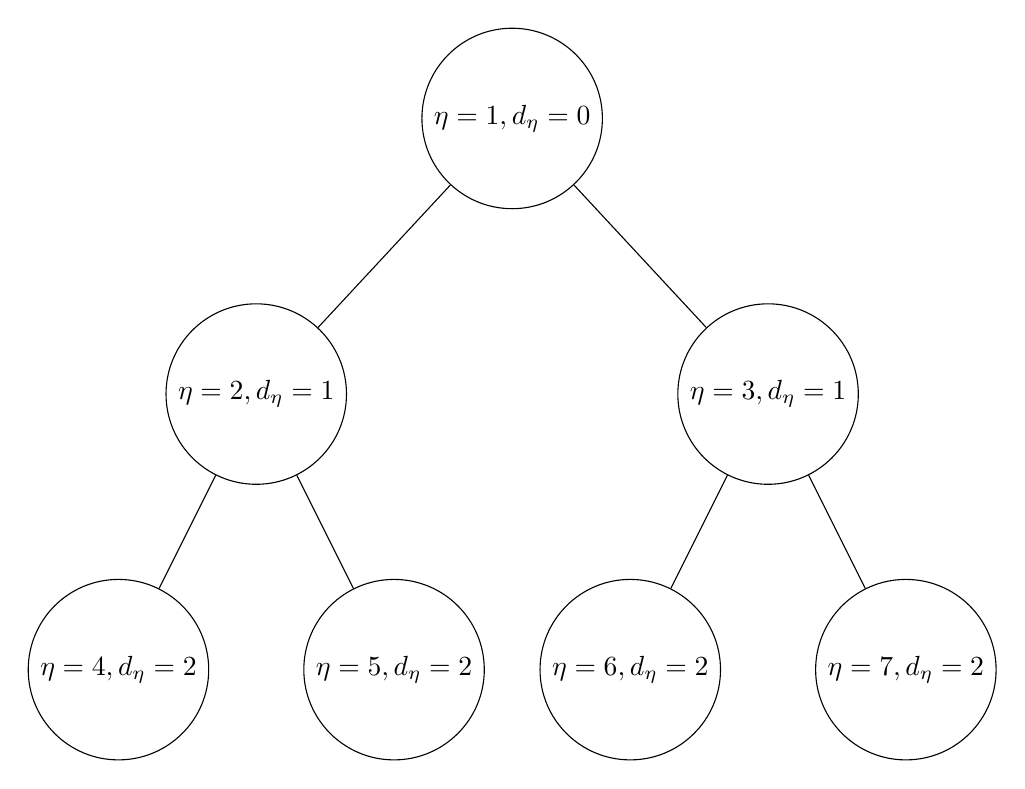
\begin{tikzpicture}
 \node [circle,draw]{$\eta=1,d_{\eta} =0$} [level distance=35mm,sibling distance=65mm]
child { node [circle,draw]{$\eta=2, d_{\eta} =1$} [level distance=35mm ,sibling distance=35mm]
child {node [circle,draw] {$\eta=4, d_{\eta} =2$}}
child {node [circle,draw]{$\eta=5, d_{\eta} =2$}}
}
child {node [circle,draw] {$\eta=3, d_{\eta} =1$} [level distance=35mm ,sibling distance=35mm]
child {node [circle,draw] {$\eta=6, d_{\eta} =2$}}
child {node [circle,draw]{$\eta=7, d_{\eta} =2$}}
};
\end{tikzpicture}

\caption{The binary heap node numbering system used in our simulations. }
\label{fig:tree_node_nums}  
\end{center}
\end{figure}
In addition to the process prior defined on the tree, we define a process prior on the selection of covariates for split rules within a tree. The function $\Pr{_{\text{rule}}}(\eta,j,r_j \vert \vec{q} )$ is decomposed into two components, one selecting the $j$th covariate which we use to propose a split at the node, and a second component selecting a specific split value ($r_j$). This corresponds to the conditional probability decomposition 

\begin{equation}\label{eqn:decomp}
\Pr{_\text{rule}}(\eta,j,r_j\vert \vec{q}) = \underbrace{\Pr{_\text{cov}}(j,\eta \vert \vec{q})}_{\text{a chosen measure}} \underbrace{\Pr{_\text{split value}}(r_j \vert j, \eta)}_{\text{Uniform}}.
\end{equation}
where the chosen measure, denoted $\Pr_{\text{cov}}(j,\eta \vert \vec{q})$ above is taken to be a discrete uniform, a Dirichlet distribution, or a Logistic Normal density in the CGM, DiVaS, and ALoVaS methods respectively. The tree prior, denoted $\Pr(\mathcal{T})$, is defined uniformly over the space of admissible trees. Exact enumeration of all admissible trees is only possible for very small values of $n$, the number of observations. The number of admissible trees is a cumulative sum of Catalan numbers less than or equal to a given depth. This sum grows at the rate $\mathcal{O}(4^n/n^{3/2})$ \cite{mattarei2009asymptotics}, the same rate as the Catalan numbers themselves, displayed in Figure \ref{fig:asymptotics}, and becomes intractable quickly. Fortunately, Markov chain Monte Carlo sampling allows us to sample from the space of trees using a Metropolis-Hastings rule with local proposals on the space of trees. We now detail the structure of the proposal functions. 

\begin{figure}[H]
  \centering
  \includegraphics[width=4in]{figures/asymptotics_plot_bw.pdf}
  \caption{Plots of the log of the number of possible trees (solid line) less than or equal to a given depth $n$, compared to exponential (45 degree line), quadratic (dash-dotted line) and linear functions (even-dashed line). Note the vertical axis is on a log scale.  }
  \label{fig:asymptotics}
\end{figure}

Given a tree $\mathcal{T}$, we sample a new tree adjacent to $\mathcal{T}$ by proposing local updates. The local updates we use are the following: 

\begin{itemize}
 \item The Grow step: choose at random one of the terminal nodes and propose to append two new child nodes with probabilities given by Equation \ref{eqn:psplit}. 
 \item The Prune step: the reverse of the grow step, a terminal node is selected at random and the selected node and that selected node's sibling are both pruned to the immediate parent of the two child nodes. The parent node becomes a terminal node. 
 \item The Change step: randomly pick an internal node and propose to change the split rule at the selected node with that of another observation, possibly on a different covariate.
  \item The Swap step: randomly select an internal node that is not the immediate parent of any terminal node and proposes to swap the split rules of the parent-child pair. Otherwise, when both child nodes split on the same covariate, both child node's rules and the parent node's rules are swapped.
  \item The Rotate step: randomly choose a left or right rotation move, each with probability $1/2$. Then a rotatable node is chosen and a rotate move is performed.
 \end{itemize}
  The rotate operation for binary trees was first introduced in Sleator and Tarjan \cite{sleator1985self} and was implemented with Bayesian decision trees by Gramacy and Lee \cite{gramacy2008bayesian}. The rotate move was originally suggested by Knight, Kustra, and Tibshirani \cite{knight1998bayesian} as another possible move that might improve mixing. A good introduction and several practical uses of the rotate move can be found in Cormen, Lieserson, Rivest, and Stein \cite{cormen2001introduction}. The proposal functions in Gramacy and Lee \cite{gramacy2008bayesian} perform a rotate move only when a swap move is proposed and the parent-child pair both split on the same covariate. We modify this and allow rotate moves to be a separate proposal function and not a special swap move case. The proposal mechanism of Chipman et al. uses the grow, prune, change and swap moves only. In addition, neither Chipman et al. \cite{chipman1998bayesian}, Denison et al. \cite{denison1998bayesian}, nor Gramacy and Lee \cite{gramacy2008bayesian} included weights on each covariate in their examples or model specifications. They sampled each covariate and each split value uniformly across all covariates. 
  
\newpage
